\documentclass{article} 
\usepackage[locale = DE,separate-uncertainty = true]{siunitx}
\usepackage{graphicx}

\begin{document} 

\section*{Erstellung eines 3D Modells der Halterung von Sensoren und Blei Platten}


Um die zuvor geplanten Halterung zu bekommen, musste ein 3D Modell erstellt werden, welches anschließend mit einem 3D Drucker hergestellt werden kann. Es handelt sich hierbei um die Eckpfosten auf welchen sowohl die Detektoren als als die Bleiplatten befestigt werden sollen. Es werden 4 Stück benötigt. 
\\
\newline
Zunächst wurden die relevanten Maße des MuPix8 Senorboards genommen. 
Hierbei ergab sich der Innendurchmesser der Befestigunslöcher zu \SI{3,1}{mm} und der Abstand von Lochmitte zu Lochmitte zu \SI{90}{mm}.
\\
Zur Erstellung des 3D Modells wird die Software Autodesk Inventor verwendet. 
In dem Programm wird zunächst eine 2D Skizze des Objektes erstellt, beginnend mit einem Rechteck mit den Maßen \SI{199,7}{mm} Länge und \SI{15}{mm} Breite. 
Nun werden im Abstand von \SI{7}{mm} Einkerbungen in das Rechteck gemacht, wobei an den Enden der Länge nach jeweils mehr Platz gelassen wird, damit die Detektoren nicht so nah am Boden liegen. 
In diese Einkerbungen werden später die Bleiplatten geschoben. 
\\
Aus der 2D Skizze wurde nun ein 3D Objekt gemacht.
 Man hat nun ein\\ 
\SI{15}{mm} $\times$ \SI{15}{mm} Quadrat als Basis des Pfostens (Siehe \ref{fig:distance_piece}). 
Auf diesen Quadraten wird nun jeweils ein Loch angebracht in welche die Schrauben der Sensoren passen um diese Dort zu befestigen. 
Die Abmessungen der Löcher sind \SI{4}{mm} Durchmesser und... %Tiefe konnte ich im Viewer nicht genau nachmessen 
\\
Schlussendlich wurde noch eine kleine Einkerbung in Form eines Pfeils in den Pfosten eingefügt, um zu sehen wo die Oberseite ist. 

\begin{figure}[h]
    \centering
    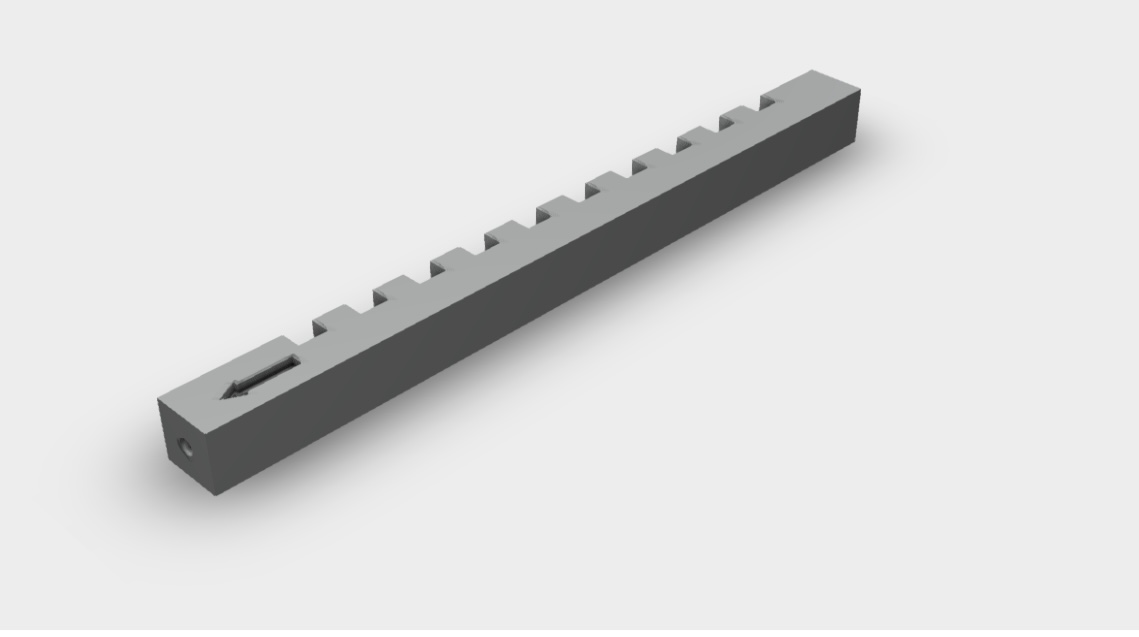
\includegraphics[width=0.8\textwidth]{Pfosten-MP8.stp.jpg}
    \caption{ Screenshot des 3D Modells}
    \label{fig:distance_piece}
\end{figure}


\end{document}
